\documentclass[a4paper, 10pt]{article}
\usepackage[utf8x]{inputenc}
\usepackage{graphicx}
\usepackage{mathenv}
\usepackage{amsmath}
\usepackage{geometry}
\geometry{hmargin = 2.5cm, vmargin = 1.5cm}

% OPENING
\title{RO05 Tp noté}
\author{Antoine Hars}

\begin{document}

\maketitle

\section*{Exercice 1}

\section*{Exercice 2}
\subsection*{1.}
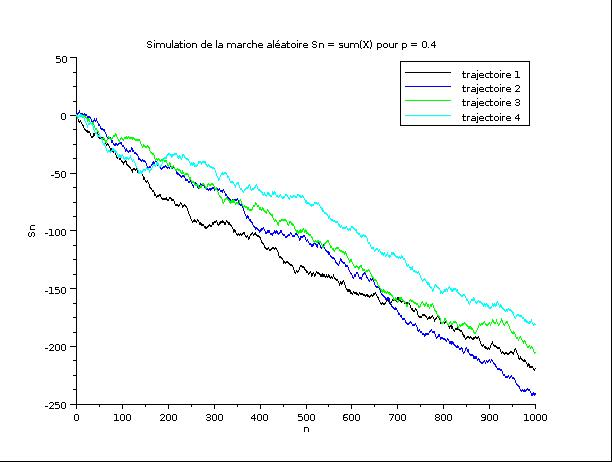
\includegraphics[height = 7cm, width = 7cm]{exercice2_plot1.jpg}
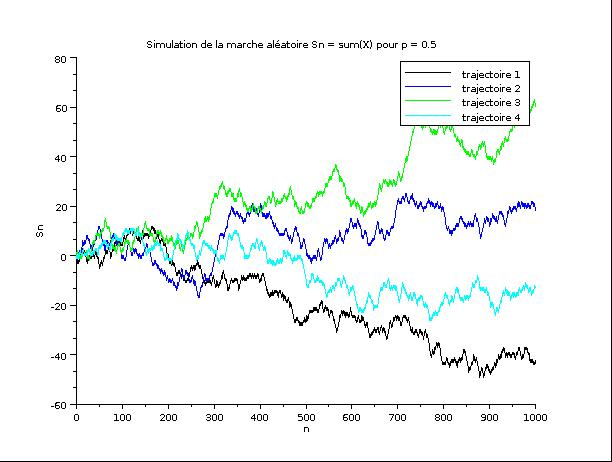
\includegraphics[height = 7cm, width = 7cm]{exercice2_plot2.jpg}\\
 On rappelle qu'on point x de E est dit récurrent si pour X0 = x, la probabilité qu'il existe n strictement positif tel que Xn = x vaut 1.
Dans ce cas, la chaîne passe presque sûrement par x une infinité de fois. Dans le cas contraîre, x est transitoire ou transient.\\
La chaine pour p = 0.5 semble récurrente alors que la chaine pour p = 0.4 semble transiente.
\subsection*{2.}
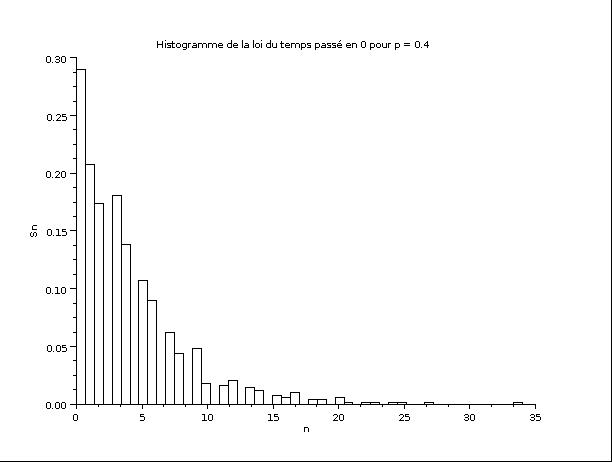
\includegraphics[height = 7cm, width = 7cm]{exercice2_histogramme1.jpg}
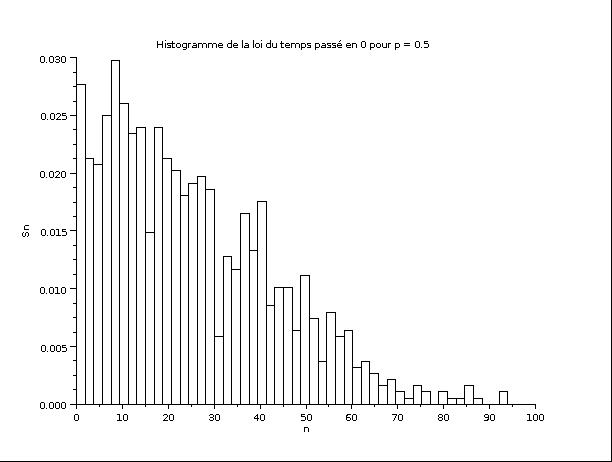
\includegraphics[height = 7cm, width = 7cm]{exercice2_histogramme2.jpg}\\
J'ai un souci sur l'exportation des graphiques, en lançant le code, on a bien les graphiques.

\section*{Exercice 3}
\subsection*{1.}
La chaine est irréductible et récurrente.\\
Une chaine est irréductible si pour tout x et y appartenant à l'espace d'états, nous avons une probabilité non nulle qu'il existe un n tel que Xn = y avec dans notre cas X0 = 0.\\

\subsection*{2.}
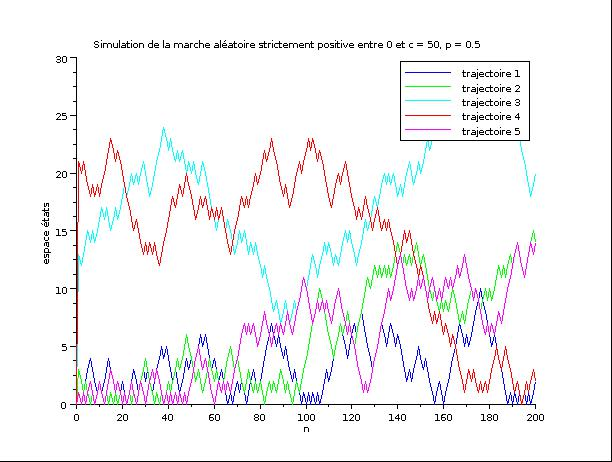
\includegraphics[height = 7cm, width = 7cm]{exercice3_plot.jpg}\\
La chaine est récurrente.

\subsection*{3.}
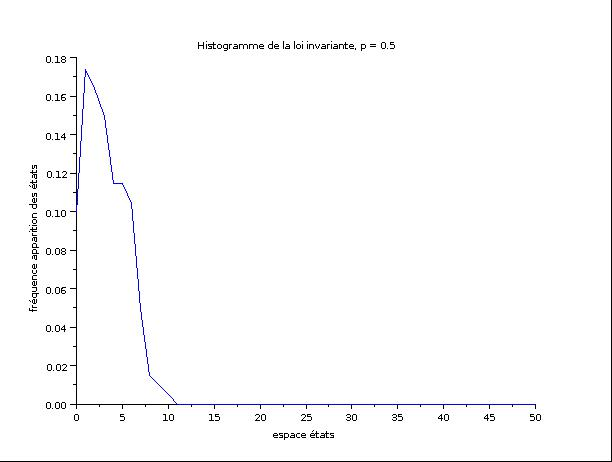
\includegraphics[height = 7cm, width = 7cm]{exercice3_histogramme.jpg}\\

\section*{Exercice 4}
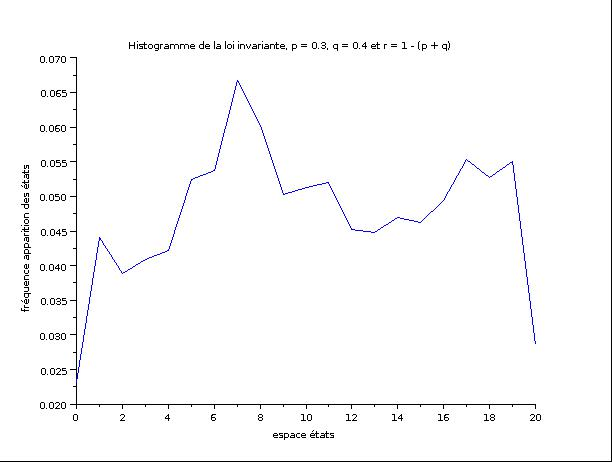
\includegraphics[height = 7cm, width = 7cm]{exercice4_histogramme.jpg}

\end{document}
